\section{Hardware Friendly Training}\label{sec:training}
In this section, we introduce our hardware-friendly training method using fixed point data and structured pruning. 

\subsection{Fixed-point Data Based Training}
Traditional CNN training relies on full-precision data, i.e. 32-bit floating point data, to guarantee a good training accuracy. However, using fixed-point data in training process can help increase the energy efficiency of training. For CNN inference, varies accelerators have been proposed with fixed point operations to increase energy efficiency. For training, using fixed point data usually suffers great model accuracy loss. Recent work~\cite{zhou2016dorefa} use narrow bit-width only for data storage in training process but have to convert the data to floating point to process addition and multiplication. In this paper, we propose a training process using both fixed point format for data storage and computation. 

In the proposed training process, every fixed-point number is represented with low bit-width (e.g. 8 bit in our implementation) together with a scaling factor. We keep a common scale for each fixed-point blob, where a blob can be the activation, weights, gradient or error of a layer. Directly using this data format will induce two problems.

The first problem is how to convert the original floating point data to the fixed point version. This means to decide the scaling factor for each data blob. One choice is to use the dynamic range of each blob as the scaling factor can keep the data precision to the best degree, but this brings extra statistic and normalization operations for each data blob in each iteration. In this work, we execute floating-point training iterations to analyze the dynamic scale of each blob and keep the scale through the rest of training process. We choose the nearest $2^n$ as the scaling factor which means data normalization can be implemented with shift operations on fixed-point data.

The second problem is the trade-off between bit-width and training accuracy. Low bit-width simplifies operations and reduce the storage consumption, but also reduce the model accuracy. Consider the small learning rate and gradient vanishing, the updated value in each iteration is small, the scaling factor of weights can be much larger than that of gradients. We use a larger bit-width to avoid gradient underflow in WG phase and only use the MSBs of weights in FP and EB phases.

\begin{figure}[tb]
  \centering 
  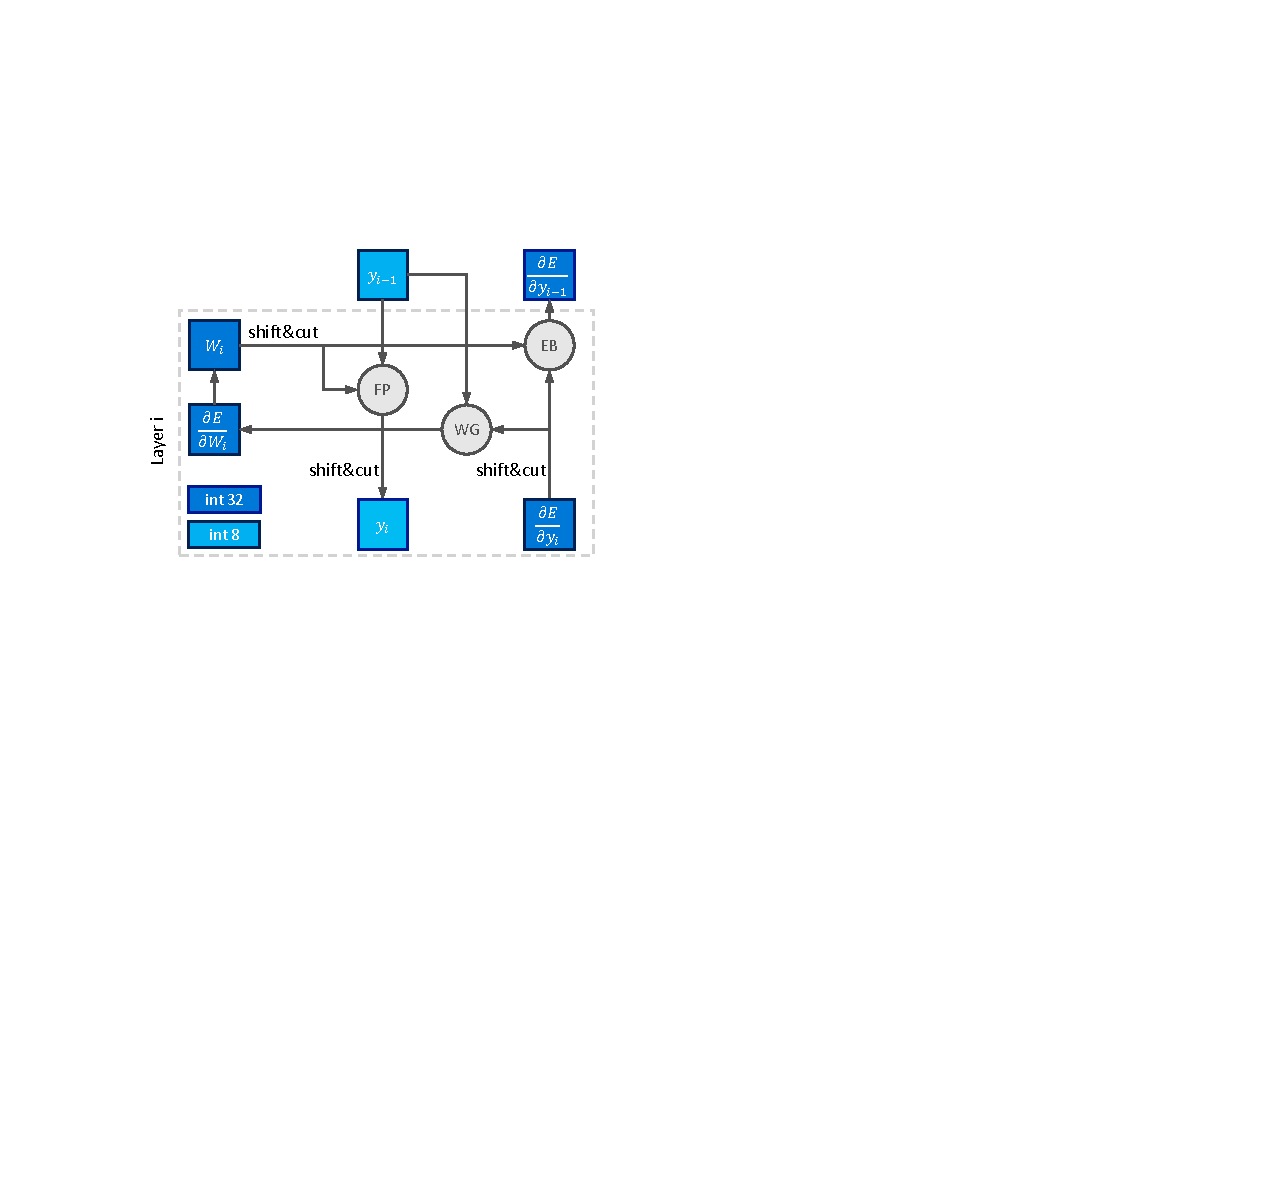
\includegraphics[width=0.8\columnwidth]{figures/fixed_train.pdf}
  \caption{Training process comparison. (a) Training with floating point data. (b) Training with fixed-point data. }
  \label{fig:fixed_train}
\end{figure}

\subsection{Structured Pruning}

We denote shape of weights as $(N, C, H, W)$. $N$ represents output channel, $C$ represents input channel, $H$ represents height, and $W$ represents weight. Compared to element-wise pruning, group-wise pruning is more efficient for hardware to realize. We choose kernel-dim pruning, which means the atomic elements during pruning is $H \times W$. L2-norm of each $H \times W$ atomic elements is used for pruning. For training with software mask matrix is used to label where is pruned and has the same shape as weights. If the weight is pruned, its mask becomes 0. Then we get sparse weights and mask matrix. 

\begin{figure}[tb]
    \centering
    
\includegraphics[width=0.8\columnwidth]{figures/prune.pdf}
    \caption{Illustration of the group-wise pruning}\label{fig:prune}
\end{figure}

\begin{table}[tb]
    \centering
    \caption{Structure of the neural network for the experiment. Sparsity denotes the ration of zeros element or convolution kernel in a layer.}
    \label{table:sparsity}
    \begin{tabular}{cccc}
    \hline
    Layer    & Type     & Dim (NxCxHxW) & Sparsity \\ \hline
    conv1    & conv     & 64x3x3x3      & 0.1      \\
    pool1    & max pool & -             & -        \\ 
    conv2    & conv     & 128x64x3x3    & 0.4      \\ 
    pool2    & max pool & -             & -        \\ 
    conv3\_1 & conv     & 256x128x3x3   & 0.3      \\ 
    conv3\_2 & conv     & 256x256x3x3   & 0.4      \\ 
    pool3    & max pool & -             & -        \\ 
    conv4\_1 & conv     & 512x256x3x3   & 0.5      \\ 
    conv4\_2 & conv     & 512x512x3x3   & 0.7      \\ 
    pool4    & max pool & -             & -        \\ 
    conv5\_1 & conv     & 512x512x3x3   & 0.9      \\ 
    conv5\_2 & conv     & 512x512x3x3   & 0.9      \\ 
    pool5    & max pool & -             & -        \\ 
    dense6   & fc       & 512x512       & 0.9      \\ 
    dense7   & fc       & 512x512       & 0.9      \\ 
    dense8   & fc       & 512x10        & 0.9      \\ 
    \hline
    \end{tabular}
\end{table}

\subsection{Software Validation}

The whole training process used in this work is as follows:
\begin{itemize}
\item Training a fixed-point model with fixed-point weights and activations using full-precision gradients on software.
\item Pruning weights and getting the mask matrix.
\item Training a fixed-point model on hardware using fixed-point gradients while keeping pruned weights zero.
\end{itemize}

The first two steps are implemented with software which use CPU and GPU as the computation platform. The third step can be executed with the proposed hardware architecture. To test the performance of the fixed-point based training method, we implemented a software version of the fixed-point data based CONV, ReLU, and pooling layers on TensorFlow.

In our implementation, the bit width of the weight buffer is set to be 24bit. The fixed scale of every gradient accumulation buffer is decided using the weight scale, the gradient scale and the learning rate after the first step. In this fine-tune stage, the fixed scales for every weight/activation/gradient blobs are fixed, and no momentum or weight decay is used. This ensures that every detail will be the same as the hardware implementation.

We perform the experiment using VGG-11\cite{Simonyan2014Very} on CIFAR-10\cite{krizhevsky2009learning} dataset. While training in the first step, the learning rate is set to 0.05 and decayed by 0.5 every 30 epochs; weight decay is set to $5 \times 10^{-4}$ and momentum is set to 0.9. We pruned model to the same sparsity in the whole experiments shown in Table~\ref{table:sparsity}. In the third training step with fixed point data, we compare the result of training with and without momentum. The accuracy is nearly the same(90.54 vs. 90.53). 

Furthermore, we also evaluate where is a good point to stop floating point training and starts fixed point training with pruned weights. Usually, we prune model when it is perfectly trained and achieves the best accuracy. But if we want to save the training time, we do not need to prune model until it perfectly trained. Table~\ref{table:prune} shows experimental results for pruning at different training stages. 

\begin{table}[tb]
    \centering
    \caption{Comparison of training result with different number of initial epochs before training}
    \label{table:prune}
    \begin{tabular}{p{0.15\columnwidth}p{0.15\columnwidth}p{0.15\columnwidth}p{0.15\columnwidth}p{0.15\columnwidth}}
    \hline
    Initial Accuracy & Initial Epochs & Fine-tune Accuracy & Fine-tune Epochs & Total Epochs \\ \hline
    %\begin{tabular}[c]{@{}c@{}}Initial\\ accuracy\end{tabular} & \begin{tabular}[c]{@{}c@{}}Initial\\ epochs\end{tabular} & \begin{tabular}[c]{@{}c@{}}Fine-tune\\ Accuracy\end{tabular} & \begin{tabular}[c]{@{}c@{}}Fine-tune\\ epoches\end{tabular} & \begin{tabular}[c]{@{}c@{}}Total\\ epoches\end{tabular} \\ \hline
    90.98   & 220   & 90.81 & 100   & 320   \\
    90.05   & 130   & 91.11 & 200   & 330   \\
    89.58   & 100   & 91.01 & 195   & 295   \\
    88.06   & 65    & 90.54 & 130   & 195   \\
    85.50   & 45    & 90.05 & 115   & 160   \\\hline
    \end{tabular}
\end{table}


The result in Table~\ref{table:prune} shows that, if we start pruning at half of training, it may cost less epochs without harming accuracy, even with small accuracy improvement. The best accuracy occurred having 130 epochs of dense training and 200 epochs of sparse training. The stopping criteria is when the learning curve starts to flatten. In this training task, 200 out of 330 epochs can be accelerated with hardware.
